\documentclass[a4paper,11pt]{article}
\usepackage{graphicx}
\usepackage[utf8]{inputenc}
\usepackage{hyperref}
\usepackage{placeins}
\usepackage{minted}


\hypersetup{
    colorlinks=true,
    linkcolor=blue,
    filecolor=black,      
    urlcolor=blue,
    citecolor=black,
}
\begin{document}

\title{
  \textbf{HP35 Calculator Report.}
}
\author{Adrian Jonsson Sjödin}
\date{Fall 2022}

\maketitle

\section*{Introduction}
The goal of this assignment is to evaluate how the time complexity changes when we apply different searching algorithms, as opposed to simply
searching through an array from start to end.
\section*{Task 1}

Set up a benchmark for the given method that searches through an unsorted array, and determine the relationship of how the time increases for a
growing number of elements in the array.

\section*{Method}

The method to benchmark was already given and required no further modification. What was left to implement for this task was solely the benchmarking
of the given method and a method creating an unsorted array. The implementation of the
benchmarking method can be seen in the code bellow.

\begin{minted}[]{java}
public static double benchmarkUnsortedSearch(int maxArraySize) {
  Random rnd = new Random();
  int[] arrayToSearch = createRandomArray(maxArraySize);
  double sum = 0;
  for (int i = 0; i < 100_000; i++) {
    int key = rnd.nextInt(arrayToSearch.length);
    long timeStart = System.nanoTime();
    searchUnsorted(arrayToSearch, key);
    sum += (double) (System.nanoTime() - timeStart) ;
  }
  return sum / 100_000;
}
\end{minted}

\section*{Result}

In fig. \ref{fig:unsortedSearch} we see a plot of how the execution time in nano seconds
increases when the array size increase. The data points are the average execution time for
an array of size $n$ over $100,000$ searches with a new random element to search for in each
search.
\begin{figure}[h!]
  \centering
  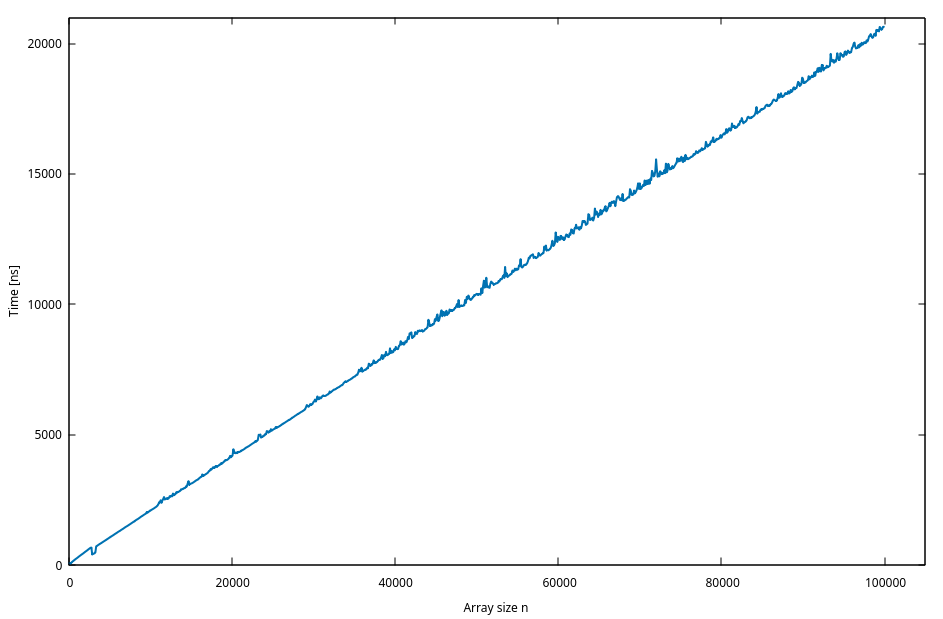
\includegraphics[width=\textwidth]{unsortedSearch.png}
  \caption{Linear search of unsorted search}
  \label{fig:unsortedSearch}
\end{figure}


\section*{Discussion}

In plot \ref{fig:unsortedSearch} we can clearly see that the time complexity for the unsorted search was $\mathcal{O}(n)$. This was expected since
the searching algorithm will have to go through each element from element $0$ up to element $n$, which is an operation of time complexity
$\mathcal{O}(n)$.

The reason why I measured the average time for a search in the benchmark test is because I generated a random key to search for each time, and
if I would have taken just the shortest amount of time it took to find said key then the result would be about the same no matter the size of the
array. This  since it is highly likely that out of the $100,000$ runs of the search algorithm for each array size, a key with a value close to, or
the same as, index $0$ would be generated. This taking the average will give a result that more accurately reflects reality.

\section*{Task 2}

Using the provided method that creates a sorted array, examine how long it will take to
find a random key in a sorted array. Furthermore estimate how long time it would
take to search through an array of one million entries.
\section*{Method}

For this task we simply need to change one line in the code for the benchmark method and
that is the line responsible for calling the method creating the array. Instead of creating
an array with random element values we create a sorted array instead. Then we just run this
array through the linear search method.

\section*{Result}

Same kind of plot as in the previous task. However for this one we only gather
data for arrays increasing in size by a 1000 instead of a 100 as in the previous
section.
\begin{figure}[h]
  \centering
  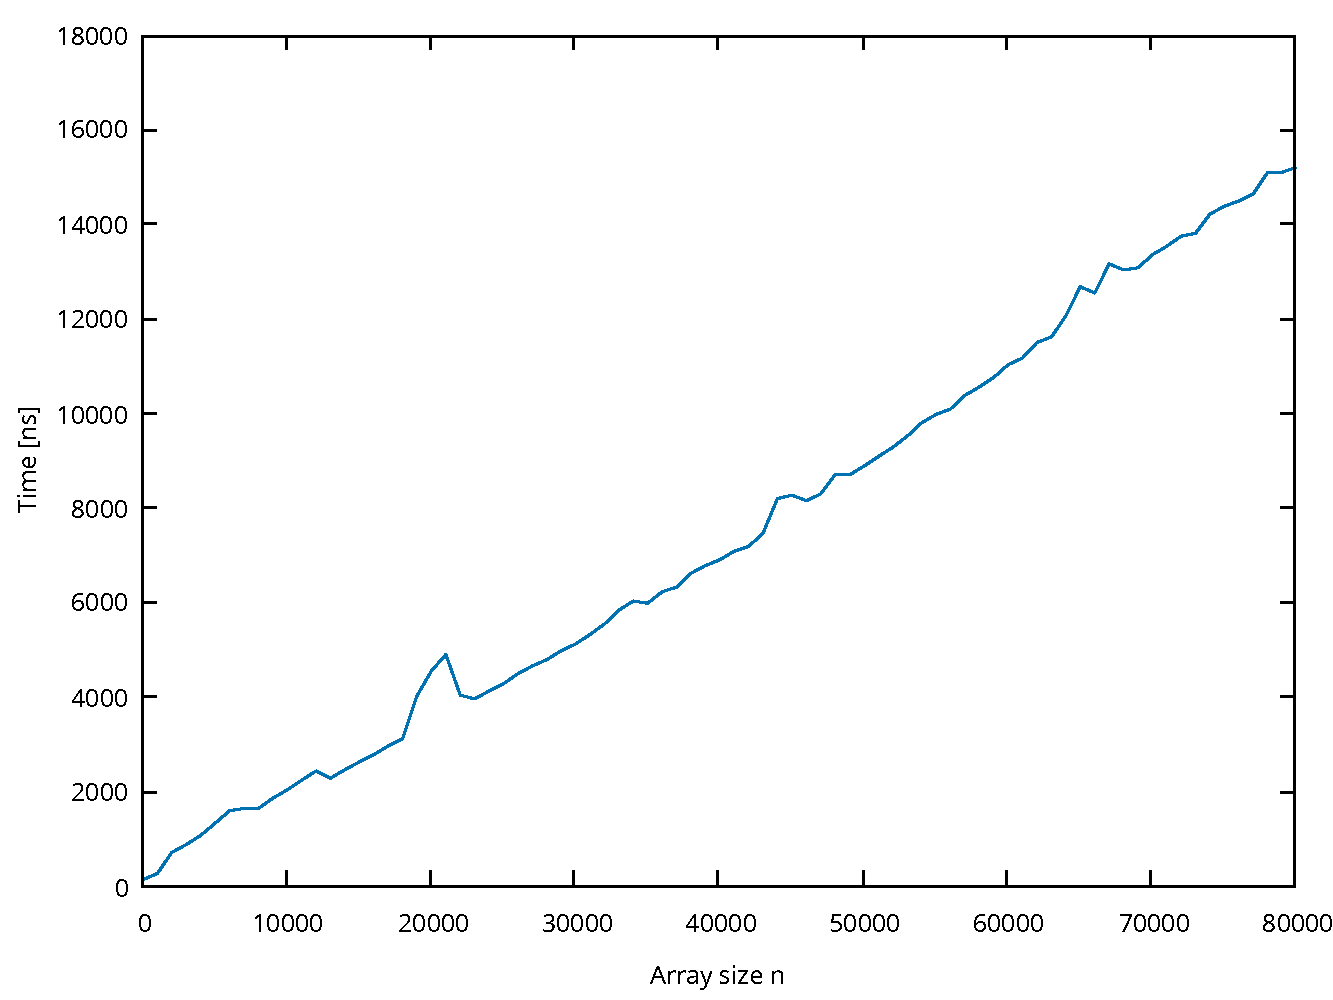
\includegraphics[width=\textwidth]{sortedLinearSearch.pdf}
  \caption{Linear search of sorted array}
  \label{fig:linearSorted}
\end{figure}
An approximate function for the graph can be derived from the linear equation $y=kx + m$,
where $k = \frac{y_2 - y_1}{x_2 - x_1}$. This give us the that the time increases approximately
as $t(n)=0.2n$ and thus it would take $200,000ns=200 \mu s$ to search through an array of size
one million.

\section*{Discussion}

As I expected the time complexity for the linear search of the sorted array is the same
as for the unsorted array, that is $\mathcal{O}(n)$. This is expected since we're still
searching through the array from start to finish and looking for a random key, and in so
doing ignoring and not taking advantage of the fact that the array is sorted. However if
we modify the linear search algorithm to stop when the current array element value is
larger than the key, it is possible to lower the time usage. It will however still be of
the order $\mathcal{O}(n)$

\section*{Task 3}

Implement the binary search algorithm and benchmark the algorithm. From the benchmark results
approximate a function that describe how the execution time increases with the size of
the array. Test the approximation by running benchmarks for arrays up to 16 million.
Lastly estimate how long it would take to search through an array of size 64 million.
\section*{Method}

The implementation of the binary search algorithm is straight forward and already described
in the assignment and the for the benchmarking we simply use the same method as already described
above, but changing which searching method we are calling.
\section*{Result}
Data from benchmark of the binary search algorithm run on arrays of size $n = 100 \to 10^6$.
Using excel we get the function $t(n)=10.5\cdot ln(n)$ describing the time-array size dependency.
\begin{figure}[h!]
  \centering
  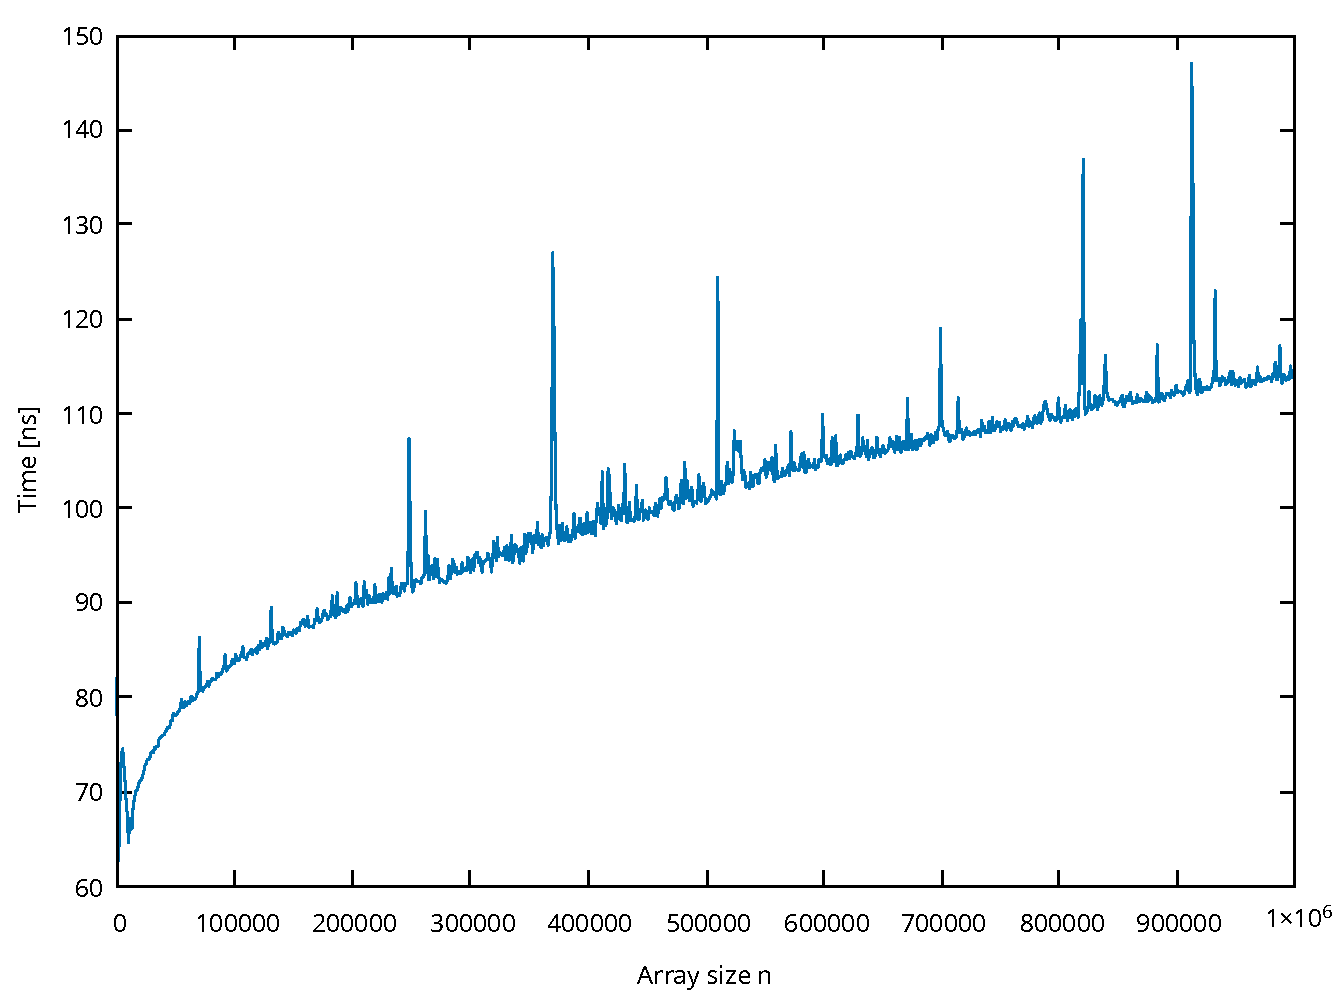
\includegraphics[width=\textwidth]{binaryLinearSearch.pdf}
  \caption{Binary search for $n =100\to 10^6$}
\end{figure}

\FloatBarrier
\section*{Discussion}
As seen in the figure above the result clearly shows that the time complexity for the binary
search algorithm is $\mathcal{O}(log(n))$. Using the approximated function we get that it
will take $10.5 \cdot ln(16\cdot 10^6)=174ns$ to search for a random element in an array
16 million long. Running a benchmark on an array of this size we get that it takes on average
$152ns$ This seems to match pretty well with the calculated result, but perhaps we should
adjust it to be $t(n)=9.5\cdot ln(n)$ instead. Using this adjusted function we get that it
will take $170ns$ to search through an array of size 64 million.

\section*{Task 4}

Search through two sorted array for duplicated elements. Do this by implementing the binary
search algorithm to try and get the time complexity down under $\mathcal{O}(n^2)$.
\section*{Method}

\section*{Result}

\section*{Discussion}

\end{document}
